
\subsection*{Adjacency Matrix Example}

%%%Insert this to get the typewriter font so it looks like a real movie script
{\ttfamily
\fontdimen2\font=0.4em
\fontdimen3\font=0.2em
\fontdimen4\font=0.1em
\fontdimen7\font=0.1em
\hyphenchar\font=`\-


\hypertarget{scripts_matrices_example}{Lets think about a graph as a mini-facebook.} In this tiny facebook there are only four people, Alice, Bob, Carl, and David. 

Suppose we have the following relationships
\begin{itemize}
\item Alice and Bob are friends.
\item Alice and Carl are friends.
\item Carl and Bob are friends.
\item David and Bob are friends.
\end{itemize}

\begin{center}
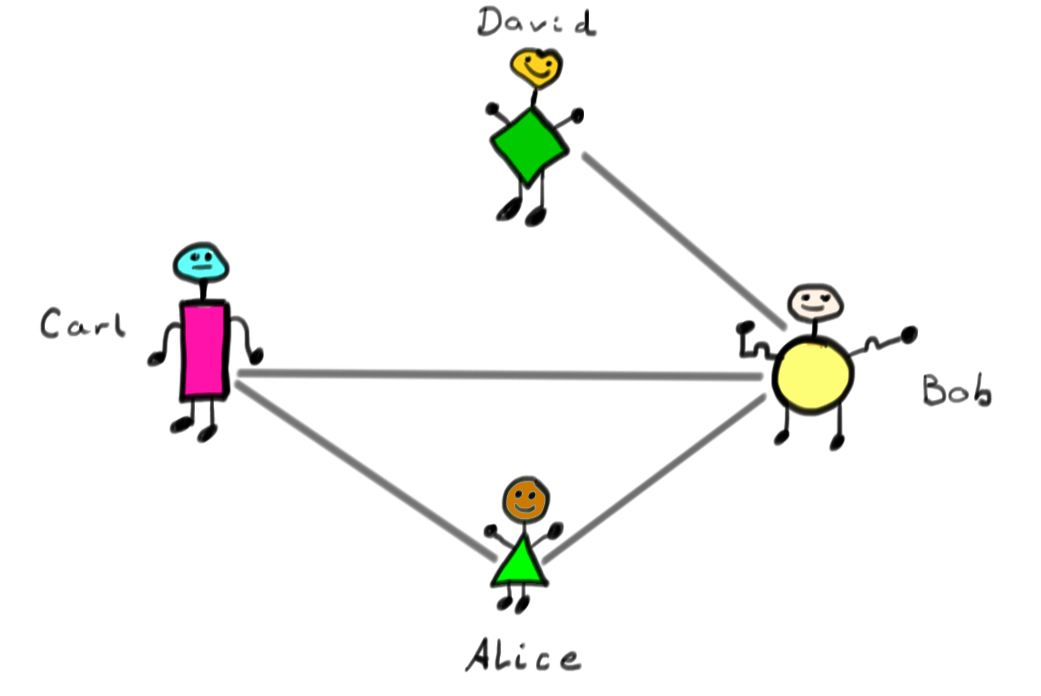
\includegraphics[alt={As explained below the dots Alice, Bob, and Carol are connected to each other.  The dots Bob and David are connected.},scale=.25]{facebook.jpg}
\end{center}

Now draw a picture where each person is a dot, and then draw a line between the dots of people who are friends. This is an example of a graph if you think of the people as nodes, and the friendships as edges.

Now lets make a $4 \times 4$ matrix, which is an adjacency matrix for the graph. Make a column and a row for each of the four people. It will look a lot like a table. When two people are friends put a 1 the row of one and the column of the other. For example Alice and Carl are friends so we can label the table below.
\begin{center}\tagpdfsetup{table/header-columns={1},table/header-rows={1}}
\begin{tabular}{r | c c c c}
 & A & B& C & D \\
 \hline
 A & & & 1 &  \\
 B & & & &  \\
 C & 1 & & &  \\
 D & & & &  \\
\end{tabular}
\end{center}

We can continue to label the entries for each friendship. Here lets assume that people are friends with themselves, so the diagonal will be all ones.

\begin{center}\tagpdfsetup{table/header-columns={1},table/header-rows={1}}
\begin{tabular}{r | c c c c}
 & A & B& C & D \\
 \hline
 A &1 &1 &1 &0  \\
 B &1 &1 &1 &1  \\
 C &1 &1 &1 &0  \\
 D &0 &1 &0 &1  \\
\end{tabular}
\end{center}

Then take the entries of this table as a matrix
\[
\left(
\begin{array}{cccc}
1 &1 &1 &0  \\
1 &1 &1 &1  \\
1 &1 &1 &0  \\
0 &1 &0 &1  \\
\end{array} \right)
\]

Notice that this table is symmetric across the diagonal, the same way a multiplication table would be symmetric. This is because on facebook friendship is symmetric in the sense that you can't be friends with someone if they aren't friends with you too. This is an example of a symmetric matrix. 

You could think about what you would have to do differently to draw a graph for something like twitter where you don't have to follow everyone who follows you. The adjacency matrix might not be symmetric then. 


} % Closing braket for font

%\newpage
